% !Mode:: "TeX:UTF-8"

\begin{frame}{第十五讲、多元函数的极值与条件极值}
	\linespread{1.5}
	\begin{enumerate}
	  \item {\bf 内容与要求}{\b (\S10.5)}
	  \begin{itemize}
	    \item 熟练掌握多元函数极值的计算和判定方法
	    \item 理解条件极值的概念
	    \item 掌握Lagrange乘子法
	    \item 了解最小二乘法
	  \vspace{1em}
	  \end{itemize}
	  \item {\bf  课后作业:}
	  \begin{itemize}
	    \item {\b 习题10.5:2,3,5,7,12}
	  \end{itemize}
	\end{enumerate}
\end{frame}

\section{多元函数的极值}

\begin{frame}{多元函数的极值}
	\linespread{1.2}\pause 
	{\bb 极值:}局部唯一的最值\pause 
	\begin{block}{{\bf 定义}\hfill}
		{\bb $n$元函数$f(\bm{x})$在$\bm{x}_0$处取最小值:}
		$f(\bm{x}_0)$有定义,且对$\bm{x}_0$某去心邻域内的任意点
		$\bm{x}$,恒有
		$f(\bm{x})>f(\bm{x}_0)$
	\end{block}
	\pause
	{\begin{center}
		\resizebox{!}{4cm}{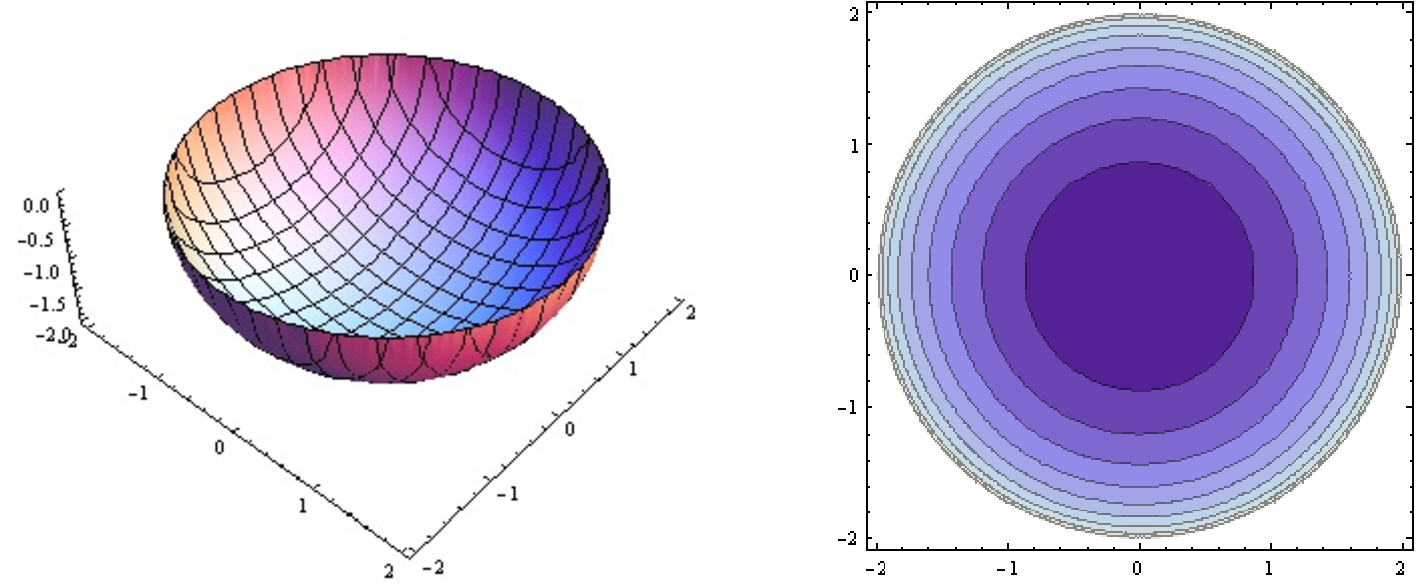
\includegraphics{./images/ch10/valley.pdf}}
	\end{center}}
\end{frame}

\begin{frame}{多元函数的极值}
	\linespread{1.2}
	{\bb 极值:}局部唯一的最值
	\begin{block}{{\bf 定义}\hfill}
		{\bb $n$元函数$f(\bm{x})$在$\bm{x}_0$处取最小值:}
		$f(\bm{x}_0)$有定义,且对$\bm{x}_0$某去心邻域内的任意点
		$\bm{x}$,恒有
		$f(\bm{x})>f(\bm{x}_0)$
	\end{block}
	{\begin{center}
		\resizebox{!}{4cm}{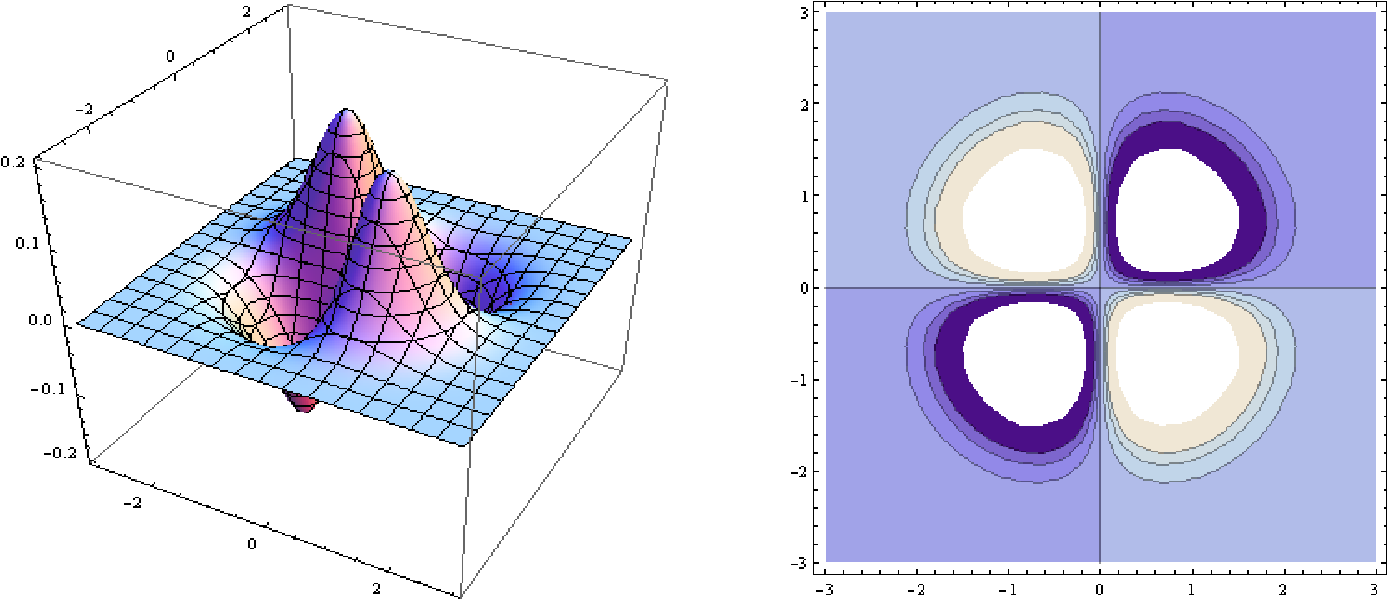
\includegraphics{./images/ch10/hill.pdf}}
	\end{center}}
\end{frame}

\begin{frame}{极值的判定}
	\linespread{1.2}
	\begin{itemize}
	  \item {\bf 一元函数的极值点:}\pause \alert{驻点}或\alert{不可导点}\pause 
	  \item {\bf 二元函数的极值点:}\pause \alert{(二维)驻点}或\alert{“不可导”点}\pause 
	\end{itemize}
	\begin{columns}
		\column{.5\textwidth}
			\begin{center}
				\resizebox{!}{4cm}{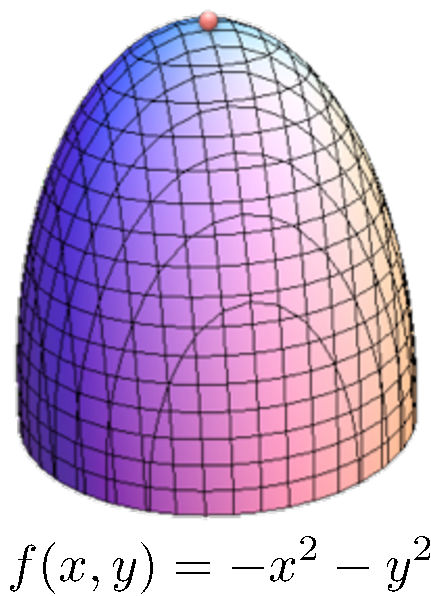
\includegraphics{./images/ch10/stayP.pdf}}\pause 
			\end{center}
		\column{.5\textwidth}
			\begin{center}
				\resizebox{!}{4cm}{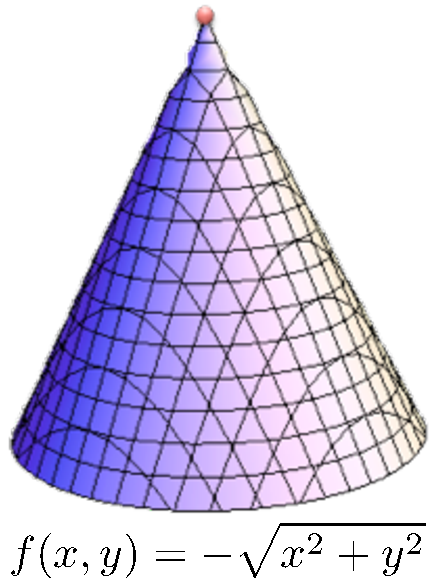
\includegraphics{./images/ch10/undevable.pdf}}
			\end{center}
	\end{columns}
\end{frame}

\begin{frame}{可微函数极值的必要条件}
	\linespread{1.2}\pause 
	\begin{block}{{\bf 定理10.5.1}\hfill}
		若可微函数$f(\bm{x})$在$\bm{x}_0$处取极值,则$\bm{x}_0$
		为$f(\bm{x})$的{\bb 驻点},即:
		$$\bigtriangledown f(\bm{x}_0)=0$$
	\end{block}
	\pause 
	\begin{block}{{\bf 推论}\hfill}
		若$f(\bm{x})$在$\bm{x}_0$处偏导连续且取极值,则对应曲面
		在该点处有水平切面。
	\end{block}
\end{frame}

\begin{frame}{驻点}
	\linespread{1.2}
	\vspace{-1em}
	$$\alert{\bigtriangledown f(\bm{x}_0)=0}$$
	\pause \vspace{-1em}
	\begin{itemize}
	  \item 可微函数的极值点必是驻点\pause 
	  \item 驻点未必是极值点\pause 
	\end{itemize}
	\vspace{-1em}
	\begin{columns}
		\column{.5\textwidth}
			\begin{center}
				\resizebox{!}{3.5cm}{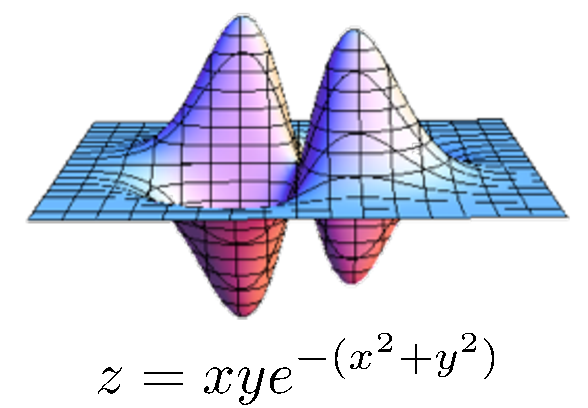
\includegraphics{./images/ch10/mhill.pdf}}\pause 
			\end{center}
		\column{.5\textwidth}
			\begin{center}
				\resizebox{!}{4cm}{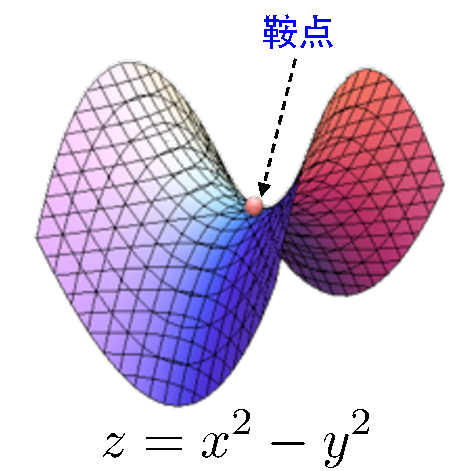
\includegraphics{./images/ch10/anhill.pdf}}
			\end{center}
	\end{columns}
\end{frame}

\begin{frame}{多元函数极值的充分条件}
	\linespread{1.2}\pause 
	\begin{block}{{\bf 定理10.5.2}\hfill}
		设$f(\bm{x})$在$\bm{x}_0$处存在二阶连续偏导数,
		$\bigtriangledown f(\bm{x}_0)=0$,则由
		$\bigtriangledown^2 f(\bm{x}_0)$正定、负定和不定
		可分别判定$\bm{x}_0$为$f(\bm{x})$的极小值、极大值
		和鞍点。\pause 
	\end{block}
	\begin{itemize}
	  \item 对多元函数而言,$\bigtriangledown f$和$\bigtriangledown^2 f$
	  类似于一元函数的一阶和二阶导数\pause 
	\end{itemize}
	\hrule
	\bigskip
	\centerline{\ba{“多元函数一/二阶可导”$\Leftrightarrow\bigtriangledown
	f$和$\bigtriangledown^2 f$存在}}
\end{frame}

\begin{frame}
	\linespread{1.2}
	\begin{block}{{\bf 定理10.5.3}(二元函数极值的充分条件)\hfill}
		$f(x,y)$在$(x_0,y_0)$二阶偏导数连续,$\bigtriangledown f(x_0,y_0)=0$,
		记$A=f\,''_{xx}(x_0,y_0),\,B=f\,''_{xy}(x_0,y_0),\,C=f\,''_{yy}(x_0,y_0)$,则
		\begin{enumerate}
		  \item 若$A>0$且$AC-B^2>0$,$(x_0,y_0)$为$f(x,y)$的极小值点;
		  \item 若$A<0$且$AC-B^2>0$,$(x_0,y_0)$为$f(x,y)$的极大值点;
		  \item $AC-B^2<0$,$(x_0,y_0)$为$f(x,y)$的鞍点。
		\end{enumerate}
	\end{block}
\end{frame}

\begin{frame}
	\linespread{1.2}
	\begin{exampleblock}{{\bf 例1}\hfill}
		求$z=-xye^{-(x^2+y^2)}$的极值。
	\end{exampleblock}\pause 
	\begin{center}
		\resizebox{!}{5cm}{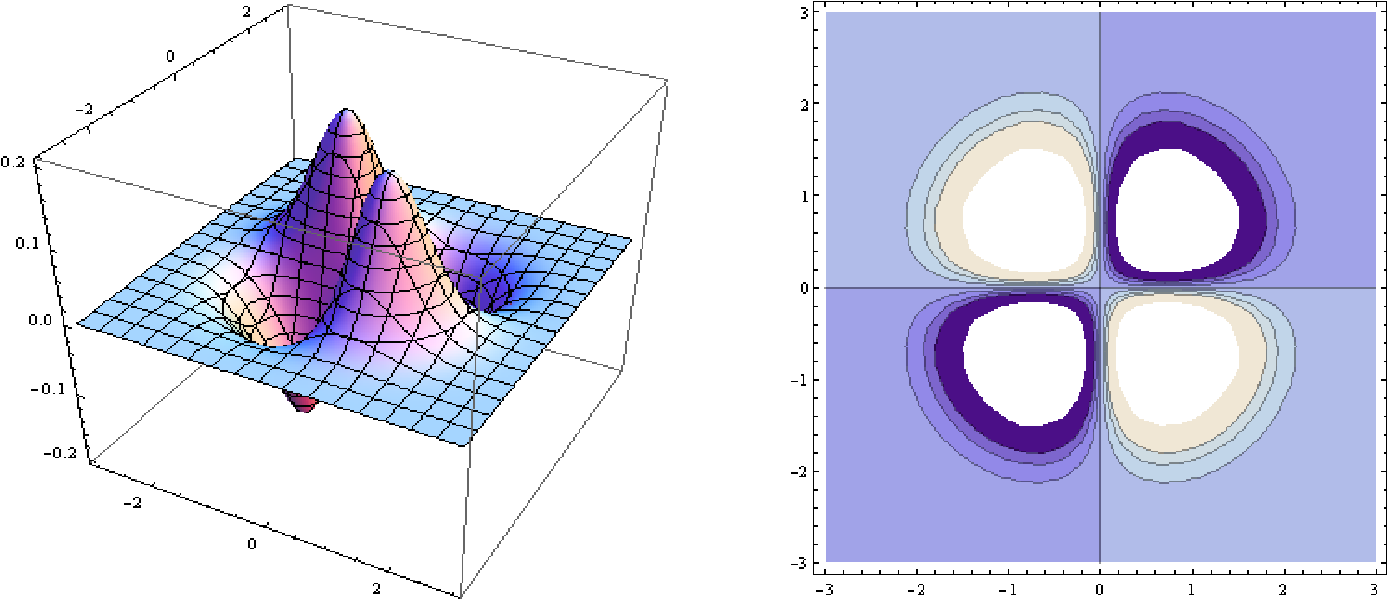
\includegraphics{./images/ch10/hill.pdf}}
	\end{center}
\end{frame}

\section{条件极值}

\begin{frame}{条件极值}
	\linespread{1.2}\pause 
	\begin{exampleblock}{{\bf 例2}\hfill}
		求函数$z=\sqrt{4-x^2-y^2}$的满足$(x-1)^2+y^2=1$的极值点。\pause 
	\end{exampleblock}
	\begin{columns}
		\column{.5\textwidth}
			\begin{center}
				\resizebox{!}{4cm}{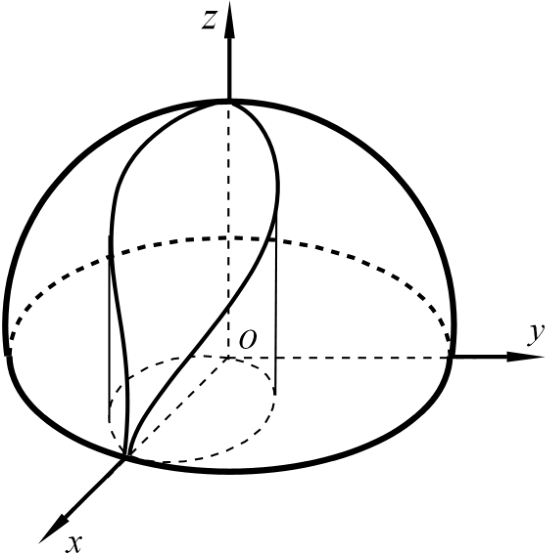
\includegraphics{./images/ch10/viviani.pdf}}\pause 
			\end{center}
		\column{.5\textwidth}
			{\bb 条件极值问题:}\pause \alert{求某个多元函数
			$z=f(\bm{x})$满足一定条件$g(\bm{x})=0$的极值}
	\end{columns}
\end{frame}

\begin{frame}{条件极值的几何意义}
	\linespread{1.2}\pause 
	{\bf 问题:}求$f(x,y)$满足$g(x,y)=0$的极值\pause 
	\bigskip
	\begin{columns}
		\column{.45\textwidth}
			\begin{center}
				\resizebox{!}{4.5cm}{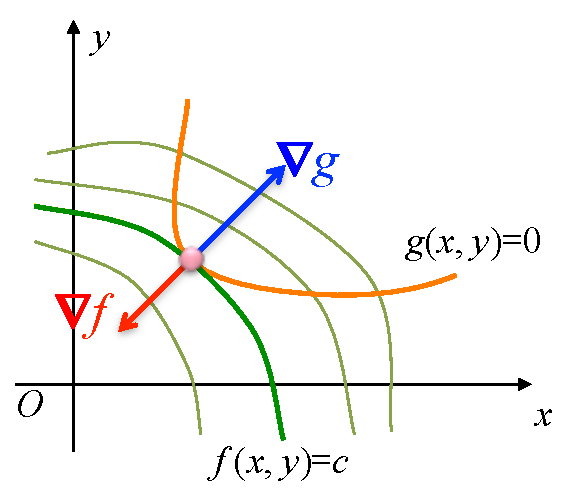
\includegraphics{./images/ch10/reshill.pdf}}\pause 
			\end{center}
		\column{.55\textwidth}
			若$f(x,y)=c$和$g(x,y)=0$光滑,则在极值点处必有
			\vspace{-1em}
			$$\alert{\bigtriangledown f // \bigtriangledown g}$$
			\pause 即存在$\lambda_0$,使得
			$$
			\alert{\left\{\begin{array}{l}
				f\,'_x(x_0,y_0)=\lambda_0g\,'_x(x_0,y_0)\\
				f\,'_y(x_0,y_0)=\lambda_0g\,'_y(x_0,y_0)
			\end{array}
			\right.}$$
	\end{columns}
\end{frame}

\begin{frame}{Lagrange乘子法}
	\linespread{1.2}\pause 
	{\bf 问题:}求函数$z=f(x,y)$满足$g(x,y)=0$的极值\pause 
	
	\bigskip
	{\bb Lagrange辅助函数:}
	$$\alert{L(x,y,\lambda)=f(x,y)+\lambda g(x,y)}$$
	\pause \vspace{-1em}
	\begin{enumerate}
	  \item $L(x,y,\lambda)$拥有相同的极值点\pause 
	  \item $L(x,y,\lambda)$的极值点$(x_0,y_0,\lambda_0)$满足\pause 
	  $$\bigtriangledown L(x_0,y_0,\lambda_0)=0$$
	\end{enumerate}
\end{frame}

\begin{frame}
	\linespread{1.2}
	\begin{exampleblock}{{\bf 例3}\hfill P166-例4}
		求函数$z=3x+4y$满足$x^2+y^2=1$的极值。\pause 
	\end{exampleblock}
	\vspace{-1em}
	\begin{center}
		\resizebox{!}{6cm}{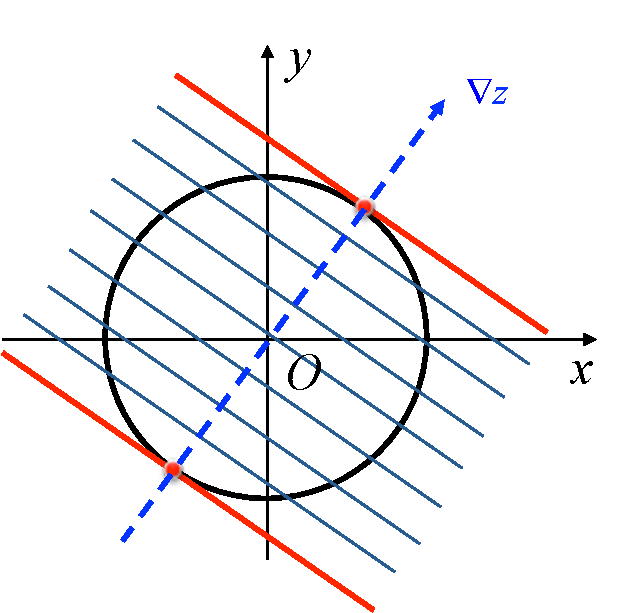
\includegraphics{./images/ch10/lagxy.pdf}}
	\end{center}
\end{frame}

\begin{frame}{更一般情形的Lagrange乘子法}
	\linespread{1.2}\pause 
	\begin{enumerate}
	  \item \ba{ 更高维:}\pause 函数$w=f(x,y,z)$满足$g(x,y,z)=0$的极值\pause 
	  
	  {\bf 解:}{\b 记$L=f(x,y,z)+\lambda g(x,y,z)$,令$\bigtriangledown L=0$}\pause 
	  \item \ba{ 更多约束:}\pause 函数$w=f(x,y,z)$满足$g_1(x,y,z)$
	  
	  $=g_2(x,y,z)=0$的极值\pause 
	  
	  {\bf 解:}{\b 记
	  \vspace{-1em}
	  $$L=f(x,y,z)+\lambda_1 g_1(x,y,z)+\lambda_2 g_2(x,y,z),$$
	  \vspace{-1em}
	  令$\bigtriangledown L=0$}
	\end{enumerate}
\end{frame}

\begin{frame}
	\linespread{1.2}
	\begin{exampleblock}{{\bf 例4}\hfill P170-例7}
		求平面$x+y+z=1$与柱面$x^2+y^2=1$上距离原点最近和最远的点。\pause 
	\end{exampleblock}
	\begin{center}
		\resizebox{!}{5cm}{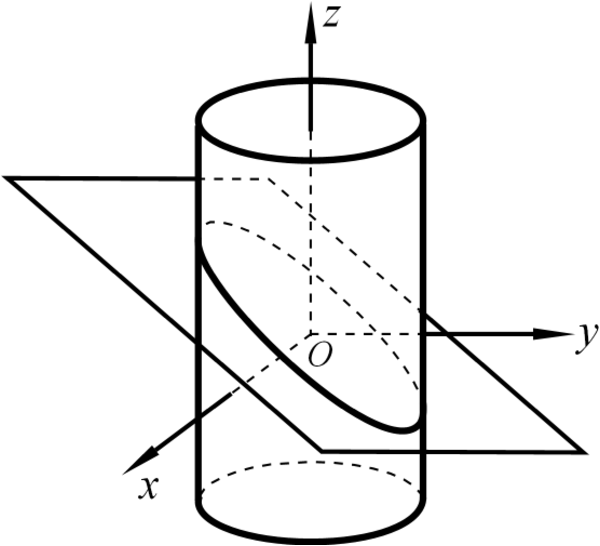
\includegraphics{./images/ch10/planeCy.pdf}}
	\end{center}
\end{frame}

\begin{frame}
	\linespread{1.2}
	\begin{exampleblock}{{\bf 例5}\hfill P169-例6}
		要制作一个表面积为$a^2$的无盖长方体盒子,
		问其长宽高各为多少时,盒子的容积最大。\pause 
	\end{exampleblock}
	\alert{
	$$x=y=\df a{\sqrt 3},\;z=\df a{2\sqrt3}$$
	$$V_{\max}=\df{a^2}{6\sqrt 3}$$
	}
\end{frame}

\begin{frame}[<+->]{小结}
	\linespread{1.5}
	\begin{enumerate}
	  \item {\bf 多元函数的极值}
	  \begin{itemize}
	    \item 必要条件:驻点或“不可导”点
	    \item 充分条件:$\bigtriangledown f=0$且
	    $\bigtriangledown^2 f=0$正(负)定
	  \end{itemize}
	  \item {\bf 条件极值}
	  \begin{itemize}
	    \item 几何意义
	    \item Lagrange乘子法
	  \end{itemize}
	\end{enumerate}
\end{frame}

%=====================================
 
% \begin{frame}{title}
% 	\linespread{1.2}
% 	\begin{exampleblock}{{\bf title}\hfill}
% 		123
% 	\end{exampleblock}
% \end{frame}
% 
% \begin{frame}{title}
% 	\linespread{1.2}
% 	\begin{block}{{\bf title}\hfill}
% 		123
% 	\end{block}
% \end{frame}